\title{Computational Photography}
\author{
        Assignment 4 - Seam Carving\\
Winter 2024
}
\date{}
\documentclass[12pt]{article}
\usepackage[margin=0.7in]{geometry}
\usepackage{graphicx}
\usepackage{float}
\usepackage{amsmath}


\begin{document}
\maketitle


\section*{Introduction}
For this assignment we are going to implement seam carving. 



\section*{Grading}
\begin{table}[h]
\begin{centering}
\begin{tabular}{|l|l|}
\hline
Theory Questions & 15pts \\
Energy Matrix & 20pts \\
Optimal Seam Discovery & 30pts\\
Optimal Seam Removal & 15pts\\
Full Removal & 20pts\\

\hline
\textbf{TOTAL} & 100pts\\
\hline
\end{tabular}
\caption{Grading Rubric}
\end{centering}
\end{table}

\newpage
\section{Theory Questions}
\begin{enumerate}

\item If the matrix below is the gradient magnitude image
$$G =
\begin{bmatrix}
2&	3&	4&	5&	1\\
1&	0&	2&	2&	1\\
4&	3&	5&	1&	2\\
4&	4&	4&	4&	6\\
4&	5&	2&	0&	2\\
2&	3&	3&	0&	3\\
\end{bmatrix}
$$

\begin{enumerate}
\item Construct the cost matrix if we assume vertical seams (10pts).

\item The cost matrix \(C\) calculated from the gradient magnitude image is given by:

\[
C =
\begin{bmatrix}
	2 & 3 & 4 & 5 & 1 \\
	3 & 2 & 5 & 3 & 2 \\
	6 & 5 & 7 & 3 & 4 \\
	9 & 9 & 7 & 7 & 9 \\
	13 & 12 & 9 & 7 & 9 \\
	14 & 12 & 10 & 7 & 10 \\
\end{bmatrix}
\]

\item What is the optimal seam (5pts)?

\item The optimal seam, representing the path of minimum cumulative energy from the top to the bottom of the image, is found to traverse the following columns in each row (using 1-based indexing):

\[
\text{seam} =
\begin{bmatrix}
	6 \\
	6 \\
	5 \\
	5 \\
	5 \\
	4 \\
\end{bmatrix}
\]

This path indicates a traversal from the bottom row, moving from the 4th column to the 5th column in the middle rows, and finally to the 6th column at the top, effectively identifying the path of least energy through the image.



\end{enumerate}

\end{enumerate}


\newpage
\section{Energy Function}
First grab two images of interest to you so that we can multiple example I/O.   To do seam carving we'll first need to compute the energy functions of your images.\\

\noindent
For each of your images, compute its energy and visualize this as an image.\\

\noindent
Some implementation details:
\begin{itemize}
\item Do this in grayscale
\item First smooth your grayscale image using a Guassian kernel prior to getting the gradients (or do this in one step).  Choose parameters that make sense for you (and report them!).
\end{itemize}

\noindent
Since you already demonstrated in prior assignments your to implement RGB to Gray, Gaussian and Gradient kernels and convolution, for this assignment \textbf{may} use Matlab functions like $conv2, rgb2gray$.  In addition, for this and subsequent parts, you \textbf{may} use Matlab's \emph{imgradxy} to compute the gradients, since we've already implemented it ourselves in prior assignments.\\

\newpage

\section{Optimal Seam}
Now that you have your energy images, we must find the optimal seam in it.\\

\noindent
Using the technique discussed in class, for each of your images, 

\begin{itemize}
\item Use its energy image to compute a seam matrix.
\item Find the optimal seam in this seam matrix via backtracing.
\item Superimpose on your color image the optimal seam in red.
\end{itemize}

\noindent
Additional Details:
\begin{itemize}
\item We will do vertical seam carving, starting at the top of the image.
\item You’ll likely have to think about how to handle the edge cases.
\end{itemize}


\newpage

\section{Remove a Seam}
Now, in each image, remove its optimal seam, thereby reducing the width of the images by one pixel.


\section{Remove all the Seams!}
Finally, let's use seam carving to reduce down to a width of zero, and show the process via a video!\\

\noindent
For each of your images, create a \textbf{video} showing the seam removal process.  Each frame of the video should depict the current color image with the current optimal seam superimposed (like in the previous part). Subsequent frames should have the previous seam removed (thus be one pixel narrower).\\

\noindent
Note:
\begin{itemize}
\item When writing your image as a frame to your video, you'll have to place its contect on a  “padded” image so that all the frames have the same size.
\item To create a movie in Matlab use the \emph{VideoWriter} class.  In addition, to keep the movies relatively small in file size, use the \emph{MPEG-4} profile for your VideoWriter object.
\end{itemize}

\newpage
\section*{Submission}
For your submission, upload to Blackboard a single zip file containing:

\begin{enumerate}
\item PDF writeup that includes:
\begin{enumerate}
\item Your answer to the theory question(s).
\item Your two original images.
\item Your two energy function images for Part 2.
\item Your two optimal seam images for Part 3.
\item Your two images with the optimal seam removed, for Part 4.
\end{enumerate}
\item A README text file (not Word or PDF) that explains
\begin{itemize}
\item Features of your program
\item Name of your entry-point script
\item Any useful instructions to run your script.
\end{itemize}
\item Your source files
\item The chosen images that you are processing.
\item The videos generated for Part 5.
\end{enumerate}

\newpage
\begin{figure}
	\centering
	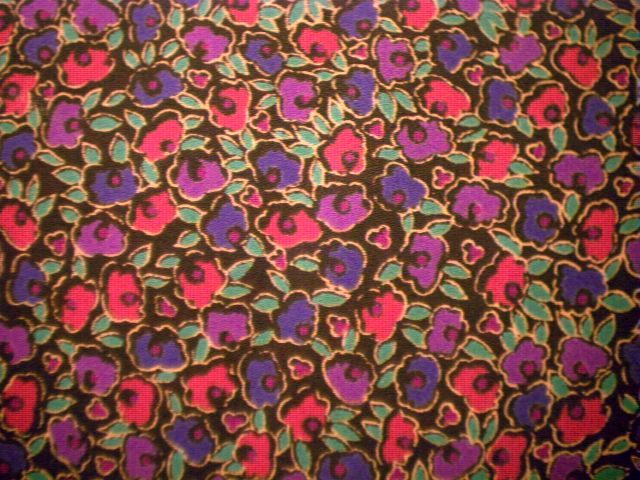
\includegraphics[width=0.7\linewidth]{fabric}
	\caption{ORIGINAL IMAGE 'fabric.png'}
	\label{fig:fabric}
\end{figure}

\begin{figure}
	\centering
	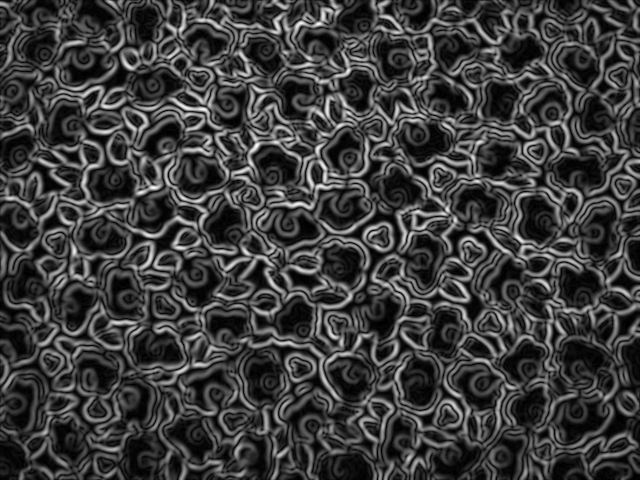
\includegraphics[width=0.7\linewidth]{fabric_energy}
	\caption{ENERGY FUNCTION IMAGE}
	\label{fig:fabricenergy}
\end{figure}

\begin{figure}
	\centering
	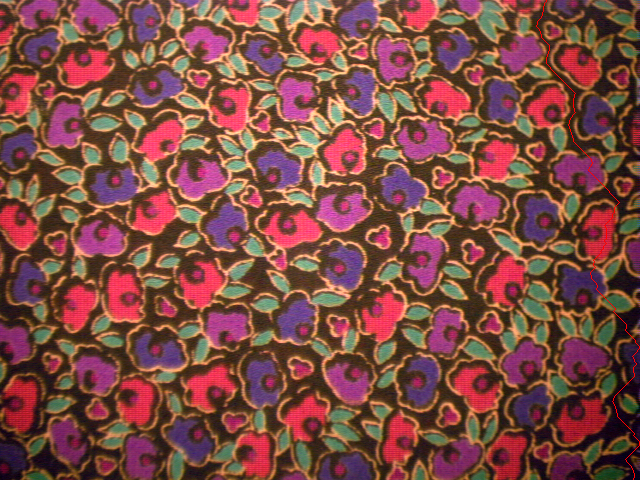
\includegraphics[width=0.7\linewidth]{fabric_seam_marked}
	\caption{OPTIMAL SEAM IMAGE}
	\label{fig:fabricseammarked}
\end{figure}

\begin{figure}
	\centering
	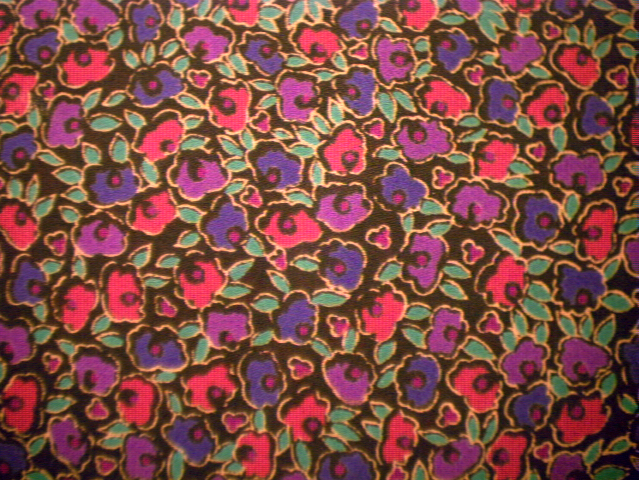
\includegraphics[width=0.7\linewidth]{fabric_seam_removed}
	\caption{OPTIMAL SEAM REMOVED}
	\label{fig:fabricseamremoved}
\end{figure}


\begin{figure}
	\centering
	\includegraphics[width=0.7\linewidth]{cameraman}
	\caption{ORIGINAL IMAGE 'cameraman.tiff'}
	\label{fig:cameraman}
\end{figure}
\begin{figure}
	\centering
	\includegraphics[width=0.7\linewidth]{cameraman_energy}
	\caption{ENERGY FUNCTION IMAGE}
	\label{fig:cameramanenergy}
\end{figure}
\begin{figure}
	\centering
	\includegraphics[width=0.7\linewidth]{cameraman_seam_marked}
	\caption{OPTIMAL SEAM IMAGE}
	\label{fig:cameramanseammarked}
\end{figure}
\begin{figure}
	\centering
	\includegraphics[width=0.7\linewidth]{cameraman_seam_removed}
	\caption{OPTIMAL SEAM REMOVED}
	\label{fig:cameramanseamremoved}
\end{figure}




\end{document}

